\newif\ifQR
%\QRtrue
\QRfalse

\documentclass[uplatex,a4paper]{jsarticle}
\usepackage[at]{easylist} 
\usepackage{eclbkbox}
\usepackage[yyyymmdd]{datetime}
\usepackage{fancyhdr}
\usepackage{multicol}

\pagestyle{fancy}
\title{T51: Strategic Japanese: Particle 1 Task Sheet}
\author{Hilofumi Yamamoto}
\date{Tokyo Institute of Technology}
%\date{2018.04.19 Ookayama\hspace*{4em}2018.04.22 Suzukakedai}
\setlength{\topmargin}{-16mm}
\setlength{\textheight}{1.3\textheight}
\lhead{\jobname}
\chead{Strategic Japanese}
\rhead{\today\,\currenttime}
\usepackage[dvipdfmx]{graphicx}	% required for `\includegraphics' (yatex added)
\begin{document}
%\maketitle
\thispagestyle{fancy}

{\noindent\LARGE Strategic Japanese: Particle 2}

\vspace*{.5\baselineskip}

%{\noindent\large Hilofumi Yamamoto --- Tokyo Institute of Technology}

You can omit particles as much as you can.\\
But there are some cases you cannot ommit them.\\
You write ``wo'' in romaji, but pronounce it ``o''.

\section{Model}

Please speak freely as natural as possible! 

\vspace*{-8\baselineskip}

\begin{flushright}
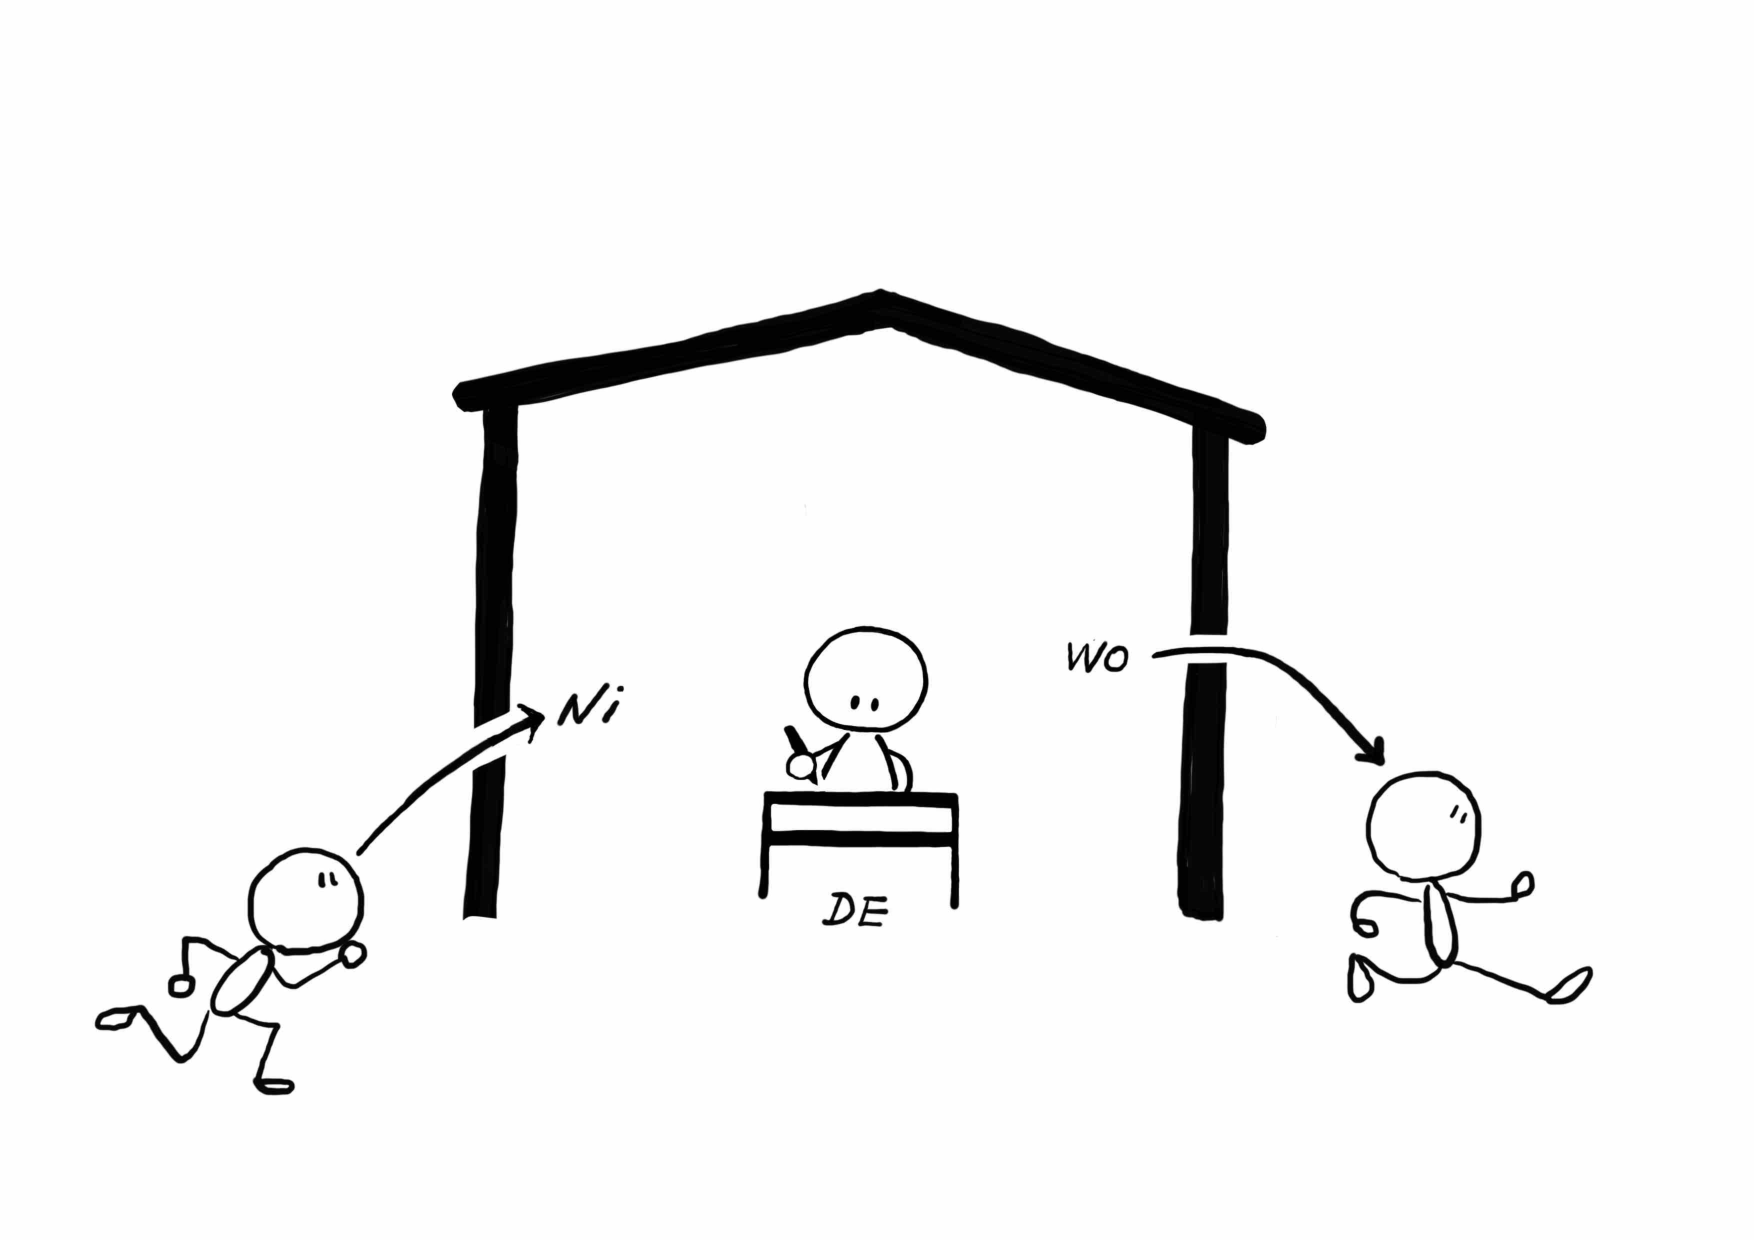
\includegraphics[trim=40 70 70 140, clip, width=.45\hsize]{toshokan-nidewo.pdf}
\end{flushright}

\vspace*{-0\baselineskip}

\begin{itemize}
   \item[A:] Nanji ni Toshokan \underline{{\bfseries ni}} tsuita? (What time did you arrive at library?) 
   \item[B:] 1 ji (ichi-ji) ni tsuita. (I arrived at 1 o'clock.)
   \item[A:] Kinou nani shita? (Yesterday, where did you do?) 
   \item[B:] Toshokan \underline{{\bfseries de}} benkyo. (I studied at library.)
   \item[A:] Nanji Toshokan \underline{{\bfseries wo}} deta? (What time did you leave library?) 
   \item[B:] 3 ji (san-ji) ni deta. (I left at 3 o'clock.)
\end{itemize}

\vspace*{-1\baselineskip}

\section{Task}
 
 Convert the following verbs into past tense and formal style.
 
 GN: past tense verb ending, {\itshape -ta} is the same as {\itshape -te}.

\begin{multicols}{2}
\begin{enumerate}
\setcounter{enumi}{-1}   
\item tsuku (arrive) $\rightarrow$ \underline{ tsuita, tsukimashita \hspace*{2em}}
 \item hairu (enter) $\rightarrow$\hrulefill
 \item yomu (read)   $\rightarrow$ \hrulefill
 \item kaku (write)  $\rightarrow$ \hrulefill
 \item deru (leave)  $\rightarrow$ \hrulefill
 \item kau (buy)     $\rightarrow$ \hrulefill
 \item dekakeru (leave) $\rightarrow$ \hrulefill
 \item suru (do)     $\rightarrow$ \hrulefill 
 \item kuru (come)   $\rightarrow$ \hrulefill
 \item mottekuru (bring) $\rightarrow$ \hrulefill
\end{enumerate}
\end{multicols}

\vspace*{-1\baselineskip}

\section{Activity}

Ask your classmates in both casual and formal style.

\begin{quote}
\begin{description}
 \item[A:] a. \underline{ Suzuki } san, m\=o toshokan b. \underline{ ni tsuita / wo deta}? 
 \item[B:] c. \underline{ Un, tsuita.}/\underline{ Uun, mada.}
\end{description}
\end{quote}
 
\begin{enumerate}
 \item a. \underline{ Suzuki\hspace{6.6zw}} b. \underline{ ni tsuita\hspace{10.8zw}} c. \underline{ mada or m\=o\hspace{10.2zw}}
 \item a. \underline{\hspace{10zw}} b. \underline{\hspace{15zw}} c. \hrulefill
 \item a. \underline{\hspace{10zw}} b. \underline{\hspace{15zw}} c. \hrulefill
 \item a. \underline{\hspace{10zw}} b. \underline{\hspace{15zw}} c. \hrulefill
 \item a. \underline{\hspace{10zw}} b. \underline{\hspace{15zw}} c. \hrulefill
% \item  a. \underline{\hspace{10zw}} b. \underline{\hspace{15zw}} c. \hrulefill
% \item  a. \underline{\hspace{10zw}} b. \underline{\hspace{15zw}} c. \hrulefill
% \item  a. \underline{\hspace{10zw}} b. \underline{\hspace{15zw}} c. \hrulefill
\end{enumerate}

%\vspace*{-1\baselineskip}

\section{Summary}

Fill in the blanks with a particle.

\begin{enumerate}
 \item daigaku \underline{\hspace{4em}} deru.
 \item ie \underline{\hspace{4em}} benky\=o shimashita.
 \item daigaku \underline{\hspace{4em}} itta?
 \item soto (outside) \underline{\hspace{4em}} tabeta?
\end{enumerate}

\ifQR
\vspace*{-6\baselineskip}
\begin{flushright}
Homework submission \includegraphics[width=24mm]{qr20180412strategic.eps}
\end{flushright}
\fi%QR

\end{document}
